%%%%%%%%%%%%%%%%%%%%%%%%%%%%%%%%%
%Preamble
%%%%%%%%%%%%%%%%%%%%%%%%%%%%%%%%%

\PassOptionsToPackage{usenames, dvipsnames, table}{xcolor}

\documentclass[]{beamer}
\usetheme{Boadilla}

%Make beamer number figures, because it doesn't by default
\setbeamertemplate{caption}[numbered]

\usepackage[english]{babel}
\usepackage[ruled, vlined]{algorithm2e}

\usepackage{amsfonts}
\usepackage{setspace, graphicx, epstopdf, amsmath}
%Do not use enumitem because this interferes with beamer drawing bullet points
\usepackage{marginnote, datetime, url, subfigure}

%Bibliography Stuff
%Use natbib even though it's old because it's compliant with journal styles
%Actual bibliography style etc are specified where you actually want it
\usepackage{natbib}

%Fluff
\linespread{1.3}

%Neural Network Packages
\usepackage{neuralnetwork}
\usepackage{xpatch}
\makeatletter
% \linklayers have \nn@lastnode instead of \lastnode,
% patch it to replace the former with the latter, and similar for thisnode
\xpatchcmd{\linklayers}{\nn@lastnode}{\lastnode}{}{}
\xpatchcmd{\linklayers}{\nn@thisnode}{\thisnode}{}{}
\makeatother

%Regression Tree
\usepackage{tikz,forest}
\usetikzlibrary{arrows.meta}

\forestset{
	.style={
		for tree={
			base=bottom,
			child anchor=north,
			align=center,
			s sep+=1cm,
			straight edge/.style={
				edge path={\noexpand\path[\forestoption{edge},thick,-{Latex}] 
					(!u.parent anchor) -- (.child anchor);}
			},
			if n children={0}
			{tier=word, draw, thick, rectangle}
			{draw, diamond, thick, aspect=2},
			if n=1{%
				edge path={\noexpand\path[\forestoption{edge},thick,-{Latex}] 
					(!u.parent anchor) -| (.child anchor) node[pos=.2, above] {Y};}
			}{
				edge path={\noexpand\path[\forestoption{edge},thick,-{Latex}] 
					(!u.parent anchor) -| (.child anchor) node[pos=.2, above] {N};}
			}
		}
	}
}

%%TODONOTE commands
\usepackage[colorinlistoftodos]{todonotes}
\newcommand{\smalltodo}[2][] {\todo[caption={#2}, size=\scriptsize,%
	fancyline,#1]{\begin{spacing}{.5}#2\end{spacing}}}
\newcommand{\rhs}[2][]{\smalltodo[color=green!30,#1]{{\bf RS:} #2}}
%%

%Graphs
\usepackage{tikz}
\usepackage{pgfplots}

%Coloured Tables


%%%%%%%%%%%%%%%%%%%%%%%%%%%%%%
%%Title and other fluff, just before document start
%%%%%%%%%%%%%%%%%%%%%%%%%%%%%%

%Hyperref apparently is a big package and causes a lot of issues, so it's recommended to load this last

\usepackage{hyperref}

%Gets rid of the neon green boxes around boxes

\usepackage[]{xcolor}

\hypersetup{
	colorlinks,
	linkcolor = {red!50!black},
	citecolor = {blue!50!black},
	urlcolor = {blue!80!black}
}

\title{Evaluation of Machine Learning in Finance}
\author{
	Ze Yu Zhong \\
	Supervisor: David Frazier
}
\institute{Monash University}


\begin{document}
	
\begin{frame}[plain]
    \maketitle
\end{frame}

\begin{frame}
	\tableofcontents
\end{frame}

%%%%%%%%%%%%%%%%%%%%%%%%%%%%%%%%%%%%%%%%%%%%%%%%%%%%
\section{Problems in Empirical Finance}
%%%%%%%%%%%%%%%%%%%%%%%%%%%%%%%%%%%%%%%%%%%%%%%%%%%%

%%%%%%%%%%%%%%%%%%%%%%%%%%%%%%%%%%%%%%%%%%%%%%%%%%%%%
%%Intereave literature review throughout this section
%%%%%%%%%%%%%%%%%%%%%%%%%%%%%%%%%%%%%%%%%%%%%%%%%%%%%

\begin{frame}
\frametitle{Background of Problems in Empirical Finance}
\begin{itemize}
	\item Regressors can be:
		\begin{itemize}
			\item Non-stationary - information now does not contain information about the future
			\item Persistent - shocks in a series have effects that last for a long time
			\item Cross sectionally correlated - regressors may seem important but are actually the result of a different underlying regressor
			\item Endogeneous - omitted variable bias, etc
		\end{itemize}
\end{itemize}
\end{frame}

\begin{frame}
\frametitle{Background Problems in Empirical Finance}
\begin{itemize}
	\item Data is not robust - structural breaks are evident in returns data, and many regressors that once performed well do not anymore
	\item Extremely large number of potential factors (regressors) that is still increasing: over 600 documented in the literature \cite{harvey_census_2019}
\end{itemize}
\end{frame}

%%%%%%%%%%%%%%%%%%%%%%%%%%%%%%%%%%%%%%%%%%%%%%%%%%%%
\section{What is Machine Learning?}
%%%%%%%%%%%%%%%%%%%%%%%%%%%%%%%%%%%%%%%%%%%%%%%%%%%%

%%%%%%%%%%%%%%%%%
%%Interweave Literature review throughout this section
%%%%%%%%%%%%%%%%%

\begin{frame}
\frametitle{What is Machine Learning?}
\begin{itemize}
	\item Statistical/Machine Learning refers to a vast set of tools for understanding data
	\item Building statistical models for predicting outputs based on inputs
	\item Find patterns in datasets
	\item Examples of procedures: Principal Components Analysis, Principal Least Squares
	\item Examples of models: Ordinary Least Squares, LASSO Regression, Generalized Linear Models, Decisions Trees, Neural Networks
\end{itemize}
\end{frame}

%%%%%%%%%%%%%%%%%%%%%%%%%%%%%%%%%%%%%%%%%%%%%%%%%%%%
\section{Why apply Machine Learning in Finance?}
%%%%%%%%%%%%%%%%%%%%%%%%%%%%%%%%%%%%%%%%%%%%%%%%%%%%

%%%%%%%%%%%%%%%%%
%%Interweave Literature review throughout this section
%%%%%%%%%%%%%%%%%

\begin{frame}
\frametitle{Why apply Machine Learning in Finance?}
\begin{itemize}
	\item Well suited for prediction
	\item Better equipped to deal with large dimensionality
	\item Capable of capturing non-linear transformations humans cannot realistically find
\end{itemize}
\end{frame}

\begin{frame}
\frametitle{Why apply Machine Learning in Finance?}
\begin{itemize}
	\item Machine Learning Algorithms have been applied successfully to solve some of the problems present
	\item \cite{kozak_shrinking_2017}, \cite{rapach_forecasting_2013}, \cite{freyberger_dissecting_2017}, among others have applied shrinkage and selection methods to identify important factors
	\item \cite{gu_empirical_2018}, \cite{hsu_finding_2014}, \cite{feng_deep_2018}, among others have constructed machine learning portfolios that historically outperform traditional portfoloios
	\item Capable of capturing non-linear transformations humans cannot realistically find
\end{itemize}
\end{frame}

%%%%%%%%%%%%%%%%%%%%%%%%%%%%%%%%%%%%%%%%%%%%%%%%%%%%
\section{Model Specification}
%%%%%%%%%%%%%%%%%%%%%%%%%%%%%%%%%%%%%%%%%%%%%%%%%%%%

\begin{frame}
\frametitle{Model Overview}
\begin{itemize}
	\item Returns are modelled as an additive error model
	\item
		\begin{equation}
		r_{i, t+1} = E(r_{i, t+1} | \mathcal{F}_t) + \epsilon_{i, t+1}
		\end{equation}
		
		where 
		
		\begin{equation}
		E(r_{i, t+1} | \mathcal{F}_t) = g^*(z_{i,t})
		\end{equation}
		
		with $g^*(z_{i,t})$ representing the model approximation using the predictor set $z_{i,t}$
\end{itemize}
\end{frame}

%%%%%%%%%%%%%%%%%%%%%%%%%%%%%%%%%%%%%%%%%%
%Sample Splitting
%%%%%%%%%%%%%%%%%%%%%%%%%%%%%%%%%%%%%%%%%%

\begin{frame}
\frametitle{Sample Splitting}
\begin{itemize}
	\item Two main approaches to dealing with temporal data
	\begin{itemize}
		\item Rolling window - training, validation, and test set lengths are fixed and move forwards in time
		\item Growing window - training set grows in size, but validation and test set lengths are fixed and move forwards in time
	\end{itemize}
	\item Hybrid approach was chosen for feasibility
	\item Define a training set, validate on the next year, forecast for the next year
	\item Increase training set by one more year and move the validation and test sets forward one year
\end{itemize}
\end{frame}

\begin{frame}
\frametitle{Sample Splitting}
\begin{figure}
	\begin{center}
		\begin{tabular}{|c|p{0.25cm}p{0.25cm}p{0.25cm}p{0.25cm}p{0.25cm}p{0.25cm}p{0.25cm}p{0.25cm}p{0.25cm}p{0.25cm}p{0.25cm}p{0.25cm}|p{0.25cm}p{0.25cm}p{0.25cm}|}
			\hline
			Set No. &&&&&&&&&&&&&&& \\
			\hline
			%%%%%%%%
			3 & \cellcolor{cyan} & \cellcolor{cyan} & \cellcolor{cyan} & \cellcolor{cyan} & \cellcolor{cyan} & \cellcolor{cyan} & \cellcolor{cyan} & \cellcolor{cyan} & \cellcolor{cyan} & \cellcolor{cyan} & \cellcolor{cyan} &
			\cellcolor{pink} & 
			\cellcolor{olive} & \cellcolor{olive} &	\cellcolor{olive} \\
			%%%%%%%%
			2 & \cellcolor{cyan} & \cellcolor{cyan} & \cellcolor{cyan} & \cellcolor{cyan} & \cellcolor{cyan} & \cellcolor{cyan} & \cellcolor{cyan} & \cellcolor{cyan} & \cellcolor{cyan} & \cellcolor{cyan} &
			\cellcolor{pink} & 
			\cellcolor{olive} & \cellcolor{olive} &	\cellcolor{olive} & \cellcolor{olive} \\
			%%%%%%%%
			1 & \cellcolor{cyan} & \cellcolor{cyan} & \cellcolor{cyan} & \cellcolor{cyan} & \cellcolor{cyan} & \cellcolor{cyan} & \cellcolor{cyan} & \cellcolor{cyan} & \cellcolor{cyan} &
			\cellcolor{pink} & 
			\cellcolor{olive} & \cellcolor{olive} &	\cellcolor{olive} & \cellcolor{olive} & \cellcolor{olive} \\
			\hline
			Year & 1 & 2 & 3 & 4 & 5 & 6 & 7 & 8 & 9 & 10 & 11 & 12 & 13 & 14 & 15\\
			\hline
		\end{tabular}
		\medskip
		\begin{tabular}{|c|p{0.25cm}|}
			\hline
			Training & \cellcolor{cyan} \\
			\hline
			Validation & \cellcolor{pink} \\
			\hline
			Test & \cellcolor{olive} \\
			\hline
		\end{tabular}
	\end{center}
	\caption{Sample Splitting Procedure}
\end{figure}
\end{frame}

%%%%%%%%%%%%%%%%%%%%%%%%%%%%%%%%%%%%%%%%%%
%Loss Functions
%%%%%%%%%%%%%%%%%%%%%%%%%%%%%%%%%%%%%%%%%%

\begin{frame}
\frametitle{Loss Functions}
\begin{itemize}
	\item Mean Absolute Error (MAE)
		\begin{equation}
		\text{MAE} = \frac{1}{n} \sum_{j = i}^{n} |y_j - \hat{y_j}|
		\end{equation}
	\item Mean Squared Error (MSE)
		\begin{align}
		\text{MSE} &= \frac{1}{n} \sum_{j = i}^{n} \left( y_j - \hat{y_j}\right) ^2
		\end{align}
	\item Huber Loss
		\begin{align}
		H(\epsilon_j = y_j - \hat{y_j};\xi) = 
		\begin{cases}
		\left( y_j - \hat{y_j}\right) ^2, 
		\quad &\text{if} \quad |y_j - \hat{y_j}| \leq \xi ; \\
		2 \xi  |y_j - \hat{y_j}| - \xi^2, 
		\quad &\text{if} \quad |y_j - \hat{y_j}| > \xi
		\end{cases}
		\end{align}
\end{itemize}
\end{frame}

\begin{frame}
\frametitle{Loss Functions}
\begin{figure}
	\begin{center}
		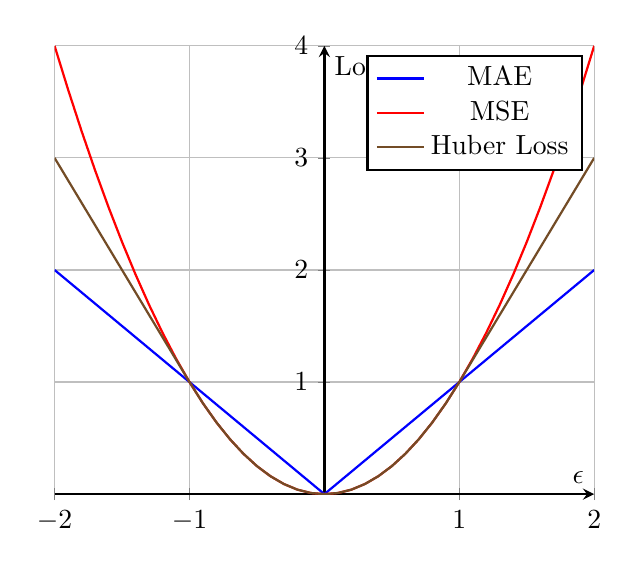
\begin{tikzpicture}
		\begin{axis}[ xlabel={$\epsilon$}, ylabel={Loss}, axis lines=middle, samples=41, grid, thick, domain=-2:2]
		\addplot+[no marks] {abs(x)};
		\addlegendentry{MAE}
		\addplot+[no marks] {x^2};
		\addlegendentry{MSE}
		\addplot+[no marks] {(2 * abs(x) - 1)*(abs(x) > 1) +
			(x^2)*(abs(x) <= 1 )};
		\addlegendentry{Huber Loss}
		\end{axis}
		\end{tikzpicture}
	\end{center}
	\caption{Illustration of MAE, MSE and Huber Loss when $\xi = 1$}
	\label{fig:loss_functions}
\end{figure}
\end{frame}

\begin{frame}
\frametitle{Models Considered}
\begin{itemize}
	\item Linear Models
	\item Penalized Linear Models (Elastic Net)
	\item Random Forests
	\item Neural Networks
\end{itemize}
\end{frame}

%%%%%%%%%%%%%%%%%%%%%%%%%%%%%%%%%%%%%%%%%%
%Linear Models
%%%%%%%%%%%%%%%%%%%%%%%%%%%%%%%%%%%%%%%%%%

\begin{frame}
\frametitle{Linear Models}
\begin{itemize}
	\item Linear Models assume that the underlying conditional expectation \( g^*(z_{i, t}) \) can be modelled as a linear function of the predictors and the parameter vector \( \theta \):
	\begin{equation}
	g(z_{i, t};\theta) = z_{i, t}' \theta
	\end{equation}
	\item Optimizing $\theta$ with respect to minimizing MSE yields the Pooled OLS estimator
	\item Limitations:
	\begin{itemize}
		\item Need to manually consider and specify non-linear interactions
		\item Struggles with high dimensionality
	\end{itemize}
\end{itemize}
\end{frame}

%%%%%%%%%%%%%%%%%%%%%%%%%%%%%%%%%%%%%%%%%%
%Penalized Linear
%%%%%%%%%%%%%%%%%%%%%%%%%%%%%%%%%%%%%%%%%%

\begin{frame}
\frametitle{Penalized Linear Models}
\begin{itemize}
	\item Penalized linear models have the same underlying statistical model as simple linear models, add a new penalty term in the loss function:
	\begin{equation}
	\mathcal{L(\theta;.)} = 
	\underset{\text{Loss Function}}{\underbrace{\mathcal{L(\theta)}}} + 
	\underset{\text{Penalty Term}}{\underbrace{\phi(\theta;.)}}
	\end{equation}
	\item Focus on the popular "elastic net" penalty  \citep{zou_regularization_2005}, which takes the form for the penalty function \( \phi(\theta;.) \):
	\begin{equation}
	\phi(\theta;\lambda,\rho) = 
	\lambda(1-\rho) \sum_{j = 1}^{P}|\theta_j| +
	\frac{1}{2} \lambda \rho \sum_{j = 1}^{P}\theta_j^2
	\end{equation}
\end{itemize}
\end{frame}

%%%%%%%%%%%%%%%%%%%%%%%%%%%%%%%%%%%%%%%%%%
%Regression Trees and Random Forests
%%%%%%%%%%%%%%%%%%%%%%%%%%%%%%%%%%%%%%%%%%

\begin{frame}
\frametitle{Regression Trees and Random Forests}
\begin{itemize}
	\item Fully non-parametric models that can capture complex multi-way interactions. 
	\item A tree "grows" in a series of iterations:
	\begin{enumerate}
		\item Make a split ("branch") along one predictor, such that it is the best split available at that stage with respect to minimizing the loss function
		\item Repeat until each observation is its own node, or until the stopping criterion is met
	\end{enumerate}
	\item The eventual model slices the predictor space into rectangular partitions, and predicts the unknown function $g^*(z_{i,t})$ with the ``average" value of the outcome variable in each partition, with repsect to minimizing the loss function	
\end{itemize}
\end{frame}

\begin{frame}
\frametitle{Regression Trees and Random Forests}
The prediction of a tree, $\mathcal{T}$, with \(K\) "leaves" (terminal nodes), and depth $L$ is

\begin{equation}
g(z_{i,t};\theta,K,L) = \sum_{k=1}^{K}\theta_k\textbf{1}_{z_{i,t}\in C_k(L)}
\end{equation}

where $C_k(L)$ is one of the $K$ partitions in the model.

Only recursive binary trees are considered. 

\end{frame}

\begin{frame}
\frametitle{Regression Trees and Random Forests}
Trees can be grown with respect to a variety of loss functions, including mean absolute error, mean squared error and Huber Loss:

\begin{equation}
H(\theta, C) = \frac{1}{|C|} \sum_{z_{i,t} \in C} L(r_{i,t+1} - \theta)
\end{equation}

where $|C|$ denotes the number of observations in set C (partition). 

Optimal prediction for each partition is the mean of the partition to minimize MSE, and the median of the partition to minimize MAE.
\end{frame}

\begin{frame}
\frametitle{Random Forests}
Trees have very low bias and high variance

They are very prone to overfitting and non-robust

Random Forests were proposed by \cite{breiman_random_2001} to address this
\begin{itemize}
	\item Create $B$ bootstrap samples
	\item Grow a highly overfit tree to each, but only using $m$ random subset of all predictors for each
	\item Average the output from all trees as an ensemble model
\end{itemize}
\end{frame}

%%%%%%%%%%%%%%%%%%%%%%%%%%%%%%%%%%%%%%%%%%%%%%%%%
%Neural Networks
%%%%%%%%%%%%%%%%%%%%%%%%%%%%%%%%%%%%%%%%%%%%%%%%%

\begin{frame}
\frametitle{Neural Networks}
Most complex type of model available

Able to capture several non-linear interactions through their many layers, hence its other name ``deep learning" 

Highly flexible and therefore often the most parameterized and least interpretable models

The scope of this paper is limited to traditional ``feed-forward" networks. 
\end{frame}

\begin{frame}
The feed forward network consists of an ``input layer" of scaled data inputs, one or more ``hidden layers" which interact and non-linearly transform the inputs, and finally an output layer that aggregates the hidden layers and transform them a final time for the final output. 

A neural network with no hidden layers reduces to already familiar regression models, such as OLS and Probit (depending on activation function chosen).



\end{frame}

\begin{frame}
\frametitle{Neural Network Specifications}
Neural networks with up to 5 hidden layers were considered. The number of neurons is each layer was chosen according to the geometric pyramid rule \citep{masters_practical_1993}

All units are fully connected: each neurons receives input from all neurons the layer before it

ReLU activation function was chosen for all hidden layers for computational speed, and hence popularity in literature:

\begin{equation}
\operatorname{ReLU}(x) = max(0, x)
\end{equation}
\end{frame}

\begin{frame}
\frametitle{Computation}
\begin{itemize}
	\item Stochastic Gradient Descent using ADAM
	\item Batch Normalization
	\item Randomize initial starting weights and biases, then average these into an ensemble model
	\item See references for specific details
\end{itemize}
\end{frame}

\begin{frame}
%Beamer hack snad uses # in a loop
%Therefore, we need to replace all # with ####
\begin{figure}
	\begin{neuralnetwork}
		%Options
		[nodespacing=9.5mm, layerspacing=18mm,
		maintitleheight=1em, layertitleheight=2em,
		height=7, toprow=false, nodesize=20pt, style={},
		title={}, titlestyle={}]
		\newcommand{\nodetextclear}[2]{}
		%use \ifnum to get different labels, such as x_n on the last neuron
		\newcommand{\nodetextx}[2]{\ifnum ####2=8 $x_n^{(0)}$ \else $x_####2^{(0)}$ \fi}
		\newcommand{\nodetexty}[2]{$y_####2$}
		%Hidden layer textcommands
		%32 neurons
		\newcommand{\nodetextxa}[2]{\ifnum ####2=7 $x_{32}^{(1)}$ \else $x_####2^{(1)}$ \fi}
		%16 neurons
		\newcommand{\nodetextxb}[2]{\ifnum ####2=6 $x_{16}^{(2)}$ \else $x_####2^{(2)}$ \fi}
		%8 neurons
		\newcommand{\nodetextxc}[2]{\ifnum ####2=5 $x_{8}^{(3)}$ \else $x_####2^{(3)}$ \fi}
		\newcommand{\nodetextxd}[2]{$x_####2^{(4)}$}
		\newcommand{\nodetextxe}[2]{$x_####2^{(5)}$}
		%Input Layer
		\inputlayer[count=8, bias=false, exclude = {7}, title=, text=\nodetextx]
		%Hidden Layer 1
		\hiddenlayer[count=7, bias=false, exclude = {6}, title=, text=\nodetextxa] 
		\linklayers[not from = {7}, not to = {6}]
		%Hidden Layer 2
		\hiddenlayer[count=6, bias=false, exclude = {5}, title=, text=\nodetextxb] 
		\linklayers[not from = {6}, not to = {5}]
		%Hidden Layer 3
		\hiddenlayer[count=5, bias=false, exclude = {4}, title=, text=\nodetextxc] 
		\linklayers[not from = {5}, not to = {4}]
		%Hidden Layer 4
		\hiddenlayer[count=4, bias=false, title=, text=\nodetextxd] 
		\linklayers[not from = {4}]
		%Hidden Layer 5
		\hiddenlayer[count=2, bias=false, title=, text=\nodetextxe] \linklayers
		%Final Layer
		\outputlayer[count=1, title=, text=\nodetexty] \linklayers
		% draw dots
		\path (L0-6) -- node{$\vdots$} (L0-8);
		\path (L1-5) -- node{$\vdots$} (L1-7);
		\path (L2-4) -- node{$\vdots$} (L2-6);
		\path (L3-3) -- node{$\vdots$} (L3-5);
	\end{neuralnetwork}
	\caption{Neural Network 5 (most complex considered)}
	\label{Neural_Network}
\end{figure}
\end{frame}

%%%%%%%%%%%%%%%%%%%%%%%%%%%%%%%%%%%%%%%%%%%%%%%%%%%%
\section{Simulation}
%%%%%%%%%%%%%%%%%%%%%%%%%%%%%%%%%%%%%%%%%%%%%%%%%%%%

\subsection{Real World Observations}
\begin{frame}
\frametitle{Real World Observations}
\begin{itemize}
	\item Though \cite{gu_empirical_2018} explore the performance of machine learning on simulated returns series, their design used factors which did not adequately capture the behaviour of stock characteristics observed in real life
	\item In particular, their specification lacks:
	\begin{itemize}
		\item Cross Sectional correlation among factors
		\item Stochastic Volatility in errors
		\item More complex interactions
		\item Multivariate time series
	\end{itemize}
\end{itemize}
\end{frame}

\subsection{Simulation Design}
\begin{frame}
\frametitle{Overall Simulation Design}
Therefore, we simulate an extension: a latent factor model with stochastic volatility for excess return, $r_{t+1}$, for $t=1,\dots,T$:

\begin{flalign}
r_{i, t+1} &= 
g\left(z_{i, t}\right) + \beta_{i,t+1}v_{t+1} + e_{i, t+1}; \\
z_{i, t} &= \left(1, x_{t}\right)^{\prime} \otimes c_{i, t}; 
\quad \beta_{i, t}=\left(c_{i 1, t}, c_{i 2, t}, c_{i 3, t}\right); \\ 
e_{i, t+1} &= 
\exp\left( \frac{\sigma_{i, t+1}^2}{2} \right) \varepsilon_{i, t+1}; \\
\sigma^2_{i,t+1} &= 
\omega + \gamma_i\sigma^2_{t,i}+w_{i,t+1}
\end{flalign}

$v_{t+1}$ is a $3\times 1$ vector of errors, $w_{i,t+1},\varepsilon_{i,t+1}$ are scalar error terms. The parameters of these were tuned such that the R squared for each individual return series was 50\% and annualized volatility 30\%.

The matrix $C_t$ is an $N\times P_c$ vector of latent factors, where the first three columns correspond to $\beta_{i,t}$, across the $1\leq i\leq N$ dimensions, while the remaining $P_c-3$ factors do not enter the return equation. The $P_x\times1$ vector $x_t$ is a $3 \times 1$ multivariate time series, and $\varepsilon_{t+1}$ is a $N\times 1$ vector of idiosyncratic errors. 

\end{frame}

\begin{frame}
\frametitle{Simulating Characteristics}
A simulation mechanism for $C_t$ that gives some correlation across the factors time was used. First consider drawing normal random numbers for each $1\leq i\leq N$ and $1\leq j\leq P_{c}$, according to 

\begin{equation}
\overline{c}_{i j, t} = \rho_{j} \overline{c}_{i j, t-1}+\epsilon_{i j, t} ;
\quad \rho_{j} \sim \mathcal{U} \left( \frac{1}{2},1 \right) 
\end{equation}

Then, define the matrix 

\begin{equation}
B:=\Lambda\Lambda' + \frac{1}{10}\mathbb{I}_{n}, \quad
\Lambda_i = (\lambda_{i1},\dots,\lambda_{i4}), \quad
\lambda_{ik}\sim N(0,1), \; k=1,\dots,4
\end{equation}
\end{frame}

\begin{frame}
\frametitle{Simulating Characteristics}
Transform this into a correlation matrix $W$ via

\begin{equation}
W = \left( \operatorname{diag}(B) \right) ^{\frac{-1}{2}}
(B)
\left( \operatorname{diag}(B) \right) ^{\frac{-1}{2}}
\end{equation}

To build in cross-sectional correlation, from the $N\times P_{c}$ matrix $\bar{C}_t$, we simulate characteristics according to

\begin{equation}
\widehat{C}_{t}=W\overline{C}_{t}
\end{equation}
\end{frame}

\begin{frame}
\frametitle{Simulating Characteristics}

Finally, the "observed" characteristics for each $1\leq i\leq N$ and for $j=1, \dots, P_{c}$ are constructed according to:

\begin{equation}
c_{i j, t} = \frac{2}{n+1} \operatorname{rank}\left(\hat{c}_{i j, t}\right) - 1.
\end{equation}

with the rank transformation normalizing all predictors to be within $[-1, 1]$ 
\end{frame}

\begin{frame}
\frametitle{Simulating Macroeconomic Time Series}
For simulation of $x_{t}$, a $3 \times 1$ multivariate time series, we consider a VAR model:
\begin{equation}
x_{t}=Ax_{t-1}+u_t, 
\quad u_t \sim N\left( \mu = (0, 0, 0)' , \Sigma = \mathbb{I}_{3}
\right)
\end{equation}
\end{frame}

\begin{frame}
\frametitle{Simulating Macroeconomic Time Series}
Consider 3 different specifications for matrix $A$:
\begin{align}
A_1 &=
	\begin{pmatrix}
	.95 & 0 & 0 \\
	0 & .95 & 0 \\
	0 & 0 & .95
	\end{pmatrix} \\
A_2 &=
	\begin{pmatrix}
	1 & 0 & .25 \\
	0 & .95 & 0 \\
	.25 & 0 &.95
	\end{pmatrix} \\
A_3 &=
	\begin{pmatrix}
	.99 & .20 & .10 \\
	.20 & .90 & -.30 \\
	.10 & -.30 & -.99
	\end{pmatrix}
\end{align}
\end{frame}

\begin{frame}
\frametitle{Simulating Return Series}
We will consider four different functions $g(\cdot)$:
\begin{flalign*}
(1)\; & g_1 \left(z_{i, t}\right)=\left(c_{i 1, t}, c_{i 2, t}, c_{i 3, t} \times x_{t}'\right) \theta_{0} \\
(2)\; & g_2 \left(z_{i, t}\right)=\left(c_{i 1, t}^{2}, c_{i 1, t} \times c_{i 2, t}, \operatorname{sgn}\left(c_{i 3, t} \times  x_{t}'\right)\right) \theta_{0} \\
(3)\; & g_3 \left(z_{i, t}\right) = \left(1[c_{i3,t}>0],c_{i 2, t}^{3}, c_{i 1, t} \times c_{i 2, t}\times 1[c_{i3,t}>0], \text{logit}\left({c}_{i 3, t} \right)\right) \theta_{0} \\
(4)\; & g_4 \left(z_{i, t}\right)=\left(\hat{c}_{i 1, t}, \hat{c}_{i 2, t}, \hat{c}_{i 3, t} \times x_{t}'\right) \theta_{0}
\end{flalign*}
$g_1 \left(z_{i, t}\right)$ is a linear specification

$g_2 \left(z_{i, t}\right)$ and $g_3 \left(z_{i, t}\right)$ is a non-linear specification with interactions

$g_4 \left(z_{i, t}\right)$ builds returns using $\hat{c}$, which are the unobserved characteristics without cross sectional correlation built in

$\theta^0$ was tuned so that the cross sectional $R^2$ was around 25\%, and the predictive $R^2$ 5\%. 

The simulation design results in $3 \times 4 = 12$ different simulated datasets, each with $N = 200$ stocks, $T = 180$ periods and $P_c = 100$ characteristics. Each design was simulated 50 times to assess the robustness of machine learning algorithms.
\end{frame}

\begin{frame}
\frametitle{Sample Splitting}
$T = 180$ monthly periods corresponds to 15 years. The training sample was set to start from $T = 108$ or 9 years, a validation set 1 year in length. The last 3 years were reserved as a test set never to be used for validation or training.
\end{frame}

\begin{frame}
\frametitle{Sample Splitting}
\begin{figure}
	\begin{center}
		\begin{tabular}{|c|p{0.25cm}p{0.25cm}p{0.25cm}p{0.25cm}p{0.25cm}p{0.25cm}p{0.25cm}p{0.25cm}p{0.25cm}p{0.25cm}p{0.25cm}p{0.25cm}|p{0.25cm}p{0.25cm}p{0.25cm}|}
			\hline
			Set No. &&&&&&&&&&&&&&& \\
			\hline
			%%%%%%%%
			3 & \cellcolor{cyan} & \cellcolor{cyan} & \cellcolor{cyan} & \cellcolor{cyan} & \cellcolor{cyan} & \cellcolor{cyan} & \cellcolor{cyan} & \cellcolor{cyan} & \cellcolor{cyan} & \cellcolor{cyan} & \cellcolor{cyan} &
			\cellcolor{pink} & 
			\cellcolor{olive} & \cellcolor{olive} &	\cellcolor{olive} \\
			%%%%%%%%
			2 & \cellcolor{cyan} & \cellcolor{cyan} & \cellcolor{cyan} & \cellcolor{cyan} & \cellcolor{cyan} & \cellcolor{cyan} & \cellcolor{cyan} & \cellcolor{cyan} & \cellcolor{cyan} & \cellcolor{cyan} &
			\cellcolor{pink} & 
			\cellcolor{olive} & \cellcolor{olive} &	\cellcolor{olive} & \cellcolor{olive} \\
			%%%%%%%%
			1 & \cellcolor{cyan} & \cellcolor{cyan} & \cellcolor{cyan} & \cellcolor{cyan} & \cellcolor{cyan} & \cellcolor{cyan} & \cellcolor{cyan} & \cellcolor{cyan} & \cellcolor{cyan} &
			\cellcolor{pink} & 
			\cellcolor{olive} & \cellcolor{olive} &	\cellcolor{olive} & \cellcolor{olive} & \cellcolor{olive} \\
			\hline
			Year & 1 & 2 & 3 & 4 & 5 & 6 & 7 & 8 & 9 & 10 & 11 & 12 & 13 & 14 & 15\\
			\hline
		\end{tabular}
		\medskip
		\begin{tabular}{|c|p{0.25cm}|}
			\hline
			Training & \cellcolor{cyan} \\
			\hline
			Validation & \cellcolor{pink} \\
			\hline
			Test & \cellcolor{olive} \\
			\hline
		\end{tabular}
	\end{center}
	\caption{Sample Splitting Procedure}
\end{figure}
\end{frame}

%%%%%%%%%%%%%%%%%%%%%%%%%%%%%%%%%%%%%%%%%%%%%%%%%%%%
\section{Real Data}
%%%%%%%%%%%%%%%%%%%%%%%%%%%%%%%%%%%%%%%%%%%%%%%%%%%%

\begin{frame}
\frametitle{Data Source}
CRSP/Compustat database for stock returns with stock level characteristics such as accounting ratios and macroeconomic factors will be queried.

Most previous studies have included decades of data in their training sample - this does not make much sense as several factors are different now

Only more recent data will be used, such as period before and after 2008 GFC
\end{frame}

%%%%%%%%%%%%%%%%%%%%%%%%%%%%%%%%%%%%%%%%%%%%%%%%%%%%
\section{Model Evaluation}
%%%%%%%%%%%%%%%%%%%%%%%%%%%%%%%%%%%%%%%%%%%%%%%%%%%%

\begin{frame}
\frametitle{Out of Sample R Squared}
Overall predictive performance for individual excess stock returns were assessed using the out of sample $R^2$:

\begin{equation}
R^2_{OOS} = 
	1 - 
	\frac{\sum_{(i, t)\in\mathcal{T}_3}(r_{i, t+1} - \widehat{r}_{i, t+1})}
	{\sum_{(i, t)\in\mathcal{T}_3} \left( r_{i, t+1} - \bar{r}_{i, t+1} \right) ^2}
\end{equation}

where $\mathcal{T}_3$ indicates that the fits are only assessed on the test subsample, which is never used for training or tuning. 
\end{frame}

\begin{frame}
\frametitle{Diebold Mariano Tests for Predictive Accuracy}
\begin{itemize}
	\item The Diebold-Mariano test (\cite{diebold_comparing_2002} and \cite{harvey_testing_1997}) compares the forecast accuracy of two forecast methods
	
	\item Different to the overall R squared metric because it tests whether or not the models' forecast accuracy is significantly different
	
	\item Tests whether or not the difference series ($d_t = e_{1t} - e_{2t}$) between two forecast methods' errors is different from zero
	
	\item As all models in this paper will be producing forecasts for an entire cross section of stocks, $e_{1t}$ and $e_{2t}$ will instead represent the average forecast errors for each model
\end{itemize}
\end{frame}

\begin{frame}
\frametitle{Diebold Mariano Tests for Predictive Accuracy}
Under the null hypothesis (forecast errors from compared models are the same):

\begin{align}
S_1^* &= \left[ 
\frac{n + 1 - 2h + n^{-1}h(h-1)}
{n} 
\right]^{1/2}S_1 ; \quad S_1^* \sim N(0,1)\\
S_1 &= \left[ 
\hat{V}(\bar{d})
\right] ^{-1/2}\bar{d} \\
\hat{\gamma}_k &= n^{-1} \sum_{t = k + 1}^{n}(d_t - \bar{d})(d_{t-k} - \bar{d}) \\
V(\bar{d}) &\approx n^{-1}\left[ 
\gamma_0 + 2 \sum_{k = 1}^{h - 1}\gamma_k
\right] 
\end{align}

where $d_t$ represents the difference series between the forecast errors of the two models $e_{1t} - e_{2t}$.
\end{frame}

\begin{frame}
\frametitle{Variable Importance}
The importance of each predictor $j$ is denoted as $VI_j$, and is defined as the reduction in predictive R-Squared from setting all values of predictor $j$ to 0, while holding the remaining model estimates fixed. 

Despite obvious limitations, this allows us to visualize which factors machine learning algorithms have determined to be important.
\end{frame}

%%%%%%%%%%%%%%%%%%%%%%%%%%%%%%%%%%%%%%%%%%%%%%%%%%%%
\section{Results}
%%%%%%%%%%%%%%%%%%%%%%%%%%%%%%%%%%%%%%%%%%%%%%%%%%%%

\begin{frame}
\frametitle{Results}

\end{frame}

%%%%%%%%%%%%%%%%%%%%%%%%%%%%%%%%%%%%%%%%%%%%%%%%%%%%
\section{References}
%%%%%%%%%%%%%%%%%%%%%%%%%%%%%%%%%%%%%%%%%%%%%%%%%%%%

%%%%%%%%%%%%%%%%%%%%%%%%%%%%%%%%%%%%%%%%%%%%%%%%%%%%
\section{Questions and Answers}
%%%%%%%%%%%%%%%%%%%%%%%%%%%%%%%%%%%%%%%%%%%%%%%%%%%%

\begin{frame}
\frametitle{Questions and Answers}
\end{frame}

\end{document}
